\section{Os espaços $\mathbb R^n$}

Uma forma usual de visualizar o conjunto $\mathbb R$ dos números reais é pensar neste como o conjunto dos pontos de uma reta.
\begin{figure}[ht]
    \centering
    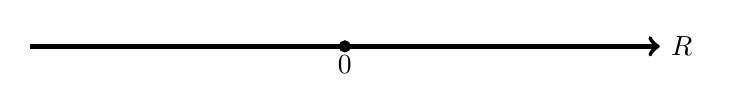
\begin{tikzpicture}
    \draw[->,ultra thick] (-4,0)--(4,0) node[right]{$\mathbb R$};
    \filldraw[black] (0,0) circle (2pt);
    \node[below] at (0,0) {0};

    \end{tikzpicture}
    \caption{A reta real.}
\end{figure}

Lembremos que $\mathbb R^2$ é o conjunto de todos os pares ordenados $(x, y)$, onde $x, y \in \mathbb R$.
Em símbolos:
\begin{equation*}
    \mathbb R^2 = \{(x, y) : x, y \in \mathbb R\}.
\end{equation*}

Em analogia à representação de $\mathbb R$ como uma reta, podemos visualizar $\mathbb R^2$ como o conjunto dos pontos de um plano Cartesiano.
\begin{figure}[ht]
    \centering
    \begin{tikzpicture}
    \draw[->,ultra thick] (-4,0)--(4,0) node[right]{$x$};
    \draw[->,ultra thick] (0,-4)--(0,4) node[above]{$y$};
    % Ponto (2,3)
    \filldraw[black] (2,3) circle (2pt);
    \node[above right] at (2,3) {$(2,3)$};
    \draw[dotted] (2,0) -- (2,3);
    \draw[dotted] (0,3) -- (2,3);
    \draw (2,0.1) -- (2,-0.1);
    \node[below] at (2,0) {2};
    \draw (0.1,3) -- (-0.1,3);
    \node[left] at (0,3) {3};
    \node[below left] at (0,0) {0};

    \end{tikzpicture}
    \caption{O plano Cartesiano.}
\end{figure}

Por sua vez, o conjunto de todas as triplas ordenadas de números reais é denotado por $\mathbb R^3$.
Em símbolos:
\begin{equation*}
    \mathbb R^3 = \{(x, y, z) : x, y, z \in \mathbb R\}.
\end{equation*}

Seguindo o padrão já comentado, podemos visualizar $\mathbb R^3$ como o conjunto dos pontos do espaço tridimensional.

\begin{figure}[ht]
    \centering
    \tdplotsetmaincoords{70}{110}
    \begin{tikzpicture}[tdplot_main_coords]
    % Eixos
    \draw[->,ultra thick] (-4,0,0)--(4,0,0) node[right]{$x$};
    \draw[->,ultra thick] (0,-4,0)--(0,4,0) node[above]{$y$};
    \draw[->,ultra thick] (0,0,-4)--(0,0,4) node[above]{$z$};
    % Ponto (2,3,1)
    \filldraw[black] (2,3,1) circle (2pt);
    \node[above right] at (2,3,1) {$(2,3,1)$};
    % Linhas pontilhadas
    \draw[dotted] (2,0,0) -- (2,3,0) -- (2,3,1);
    \draw[dotted] (0,3,0) -- (2,3,0);
    \draw[dotted] (2,0,0) -- (2,0,1) -- (2,3,1);
    \draw[dotted] (0,0,1) -- (2,0,1);
    % Marcas nos eixos
    \draw (2,0.1,0) -- (2,-0.1,0);
    \node[below] at (2,0,0) {2};
    \draw (0.1,3,0) -- (-0.1,3,0);
    \node[left] at (0,3,0) {3};
    \draw (0.1,0,1) -- (-0.1,0,1);
    \node[left] at (0,0,1) {1};
    \node[below left] at (0,0,0) {0};

    \end{tikzpicture}
    \caption{O espaço tridimensional.}
\end{figure}

No geral, para $n\geq 4$, o conjunto $\mathbb R^n$ é definido como o conjunto de todas as $n$-tuplas ordenadas de números reais:
\begin{equation*}
    \mathbb R^n = \{(x_1, \ldots, x_n) : x_1, \ldots, x_n \in \mathbb R\}.
\end{equation*}

Tal conjunto não possui uma representação gráfica simples a estilo dos anteriores.
Porém, a teoria desenvolvida para $\mathbb R^n$ é uma extensão natural da teoria desenvolvida para $\mathbb R$ e $\mathbb R^2$, e possui amplas aplicações práticas e teóricas.
\section{Operações em $\mathbb R^n$}

Algumas operações importantes em $\mathbb R^n$ incluem as seguintes.

\begin{definition}
    Sejam $v=(x_1, \ldots, x_n)$ e $w=(y_1, \ldots, y_n)$ dois vetores em $\mathbb R^n$, e $\alpha \in \mathbb R$ um escalar.
    A \emph{soma} $v+w$ é definida como:
    \begin{equation*}
        v+w =(x_1, \ldots, x_n)+(y_1, \ldots, y_n)=(x_1+y_1, \ldots, x_n+y_n).
    \end{equation*}
    A \emph{multiplicação por escalar} $\alpha v$ é definida como:
    \begin{equation*}
        \alpha v = \alpha (x_1, \ldots, x_n) = (\alpha x_1, \ldots, \alpha x_n).
    \end{equation*}
    O \emph{produto escalar} $v \cdot w$ é definido como:
    \begin{equation*}
        v \cdot w = (x_1, \ldots, x_n) \cdot (y_1, \ldots, y_n) = x_1y_1 + \ldots + x_ny_n=\sum_{i=1}^n x_iy_i.
    \end{equation*}
    A \emph{norma} de um vetor $v$ é definida como:
    \begin{equation*}
        \|v\| = \sqrt{v\cdot v}=\sqrt{x_1^2 + \ldots + x_n^2} = \sqrt{\sum_{i=1}^n x_i^2}.
    \end{equation*}
\end{definition}

Vamos lembrar de importantes interpretações geométricas destas operações.

Lembremos que um ponto do espaço $\mathbb R^n$ pode ser visto como um vetor que parte da origem $(0, \ldots, 0)$ até o ponto $(x_1, \ldots, x_n)$.

A soma dos vetores $v=(3, 2)$ e $w=(-1, 1)$ pode ser visualizada como o vetor com início da origem e fim no ponto obtido posicionando-se o vetor $w$ com início no ponto final do vetor $v$, conforme ilustrado abaixo.

\begin{figure}[ht]
    \centering
    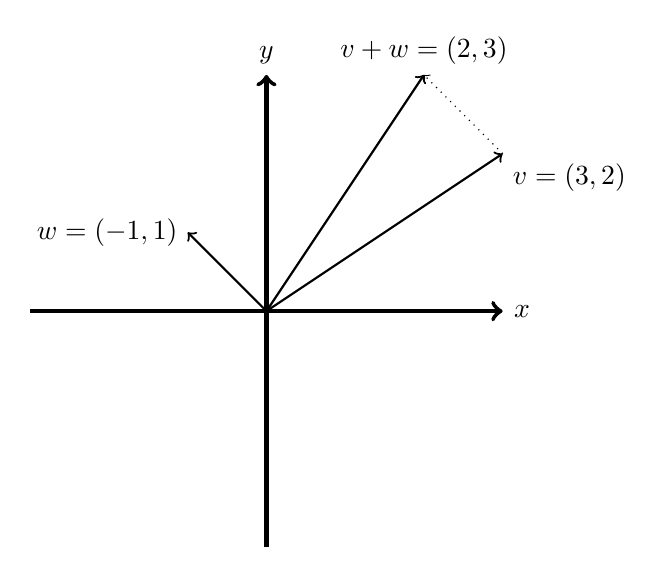
\begin{tikzpicture}
    \draw[->,ultra thick] (-3,0)--(3,0) node[right]{$x$};
    \draw[->,ultra thick] (0,-3)--(0,3) node[above]{$y$};
    % Vetor v=(3,2)
    \draw[->,thick] (0,0) -- (3,2) node[below right]{$v=(3,2)$};
    % Vetor w=(-1,1)
    \draw[->,thick] (0,0) -- (-1,1) node[left]{$w=(-1,1)$};
    % Vetor cópia w=(-1,1)
    \draw[->,dotted] (3,2) -- (2,3);
    % Soma v+w
    \draw[->,thick] (0,0) -- (2,3) node[above, align=left]{$v+w=(2,3)$};
    \end{tikzpicture}
    \caption{Soma de vetores em $\mathbb R^2$.}
\end{figure}
O produto escalar de $v=(1, 2)$ por $2$ e por $-2$ correspondem a, respectivamente, multiplicar o comprimento do vetor $v$ pelo fator $2$, mantendo a direção e sentido, e invertendo o sentido.

\begin{figure}[ht]
    \centering
    \begin{tikzpicture}
    \draw[->,ultra thick] (-3,0)--(3,0) node[right]{$x$};
    \draw[->,ultra thick] (0,-3)--(0,3) node[above]{$y$};

    % Vetor 2v
    \draw[->,thick, draw=blue] (0,0) -- (2,4) node[above right]{$2v=(2,4)$};
    % Vetor 2v
    \draw[->,thick, draw=red] (0,0) -- (-2,-4) node[above right]{$-2v=(-2,-4)$};
    % Vetor v=(1,2)
    \draw[->,thick] (0,0) -- (1,2) node[below right]{$v=(1,2)$};
    \end{tikzpicture}
    \caption{Produto por escalar em $\mathbb R^2$.}
\end{figure}

A norma de um vetor $v=(x_1, \ldots, x_n)$ é o comprimento do vetor que parte da origem até o ponto $(x_1, \ldots, x_n)$ utilizando-se a métrica  usual (Euclidiana) em $\mathbb R^n$.

O produto escalar pode ser utilizado para decidir-se ortogonalidade entre vetores.
É fato conhecido que vale a recíproca do Teorema de Pitágoras: se $\triangle BAC$ é um triângulo, então o ângulo $\angle ABC$ é reto se, e somente se, sendo $a, b, c$ respectivamente as medidas dos segmentos $\overline{BC}, \overline{AC}, \overline{AB}$, temos que $a^2=b^2+c^2$.

\begin{figure}[ht]
    \centering
    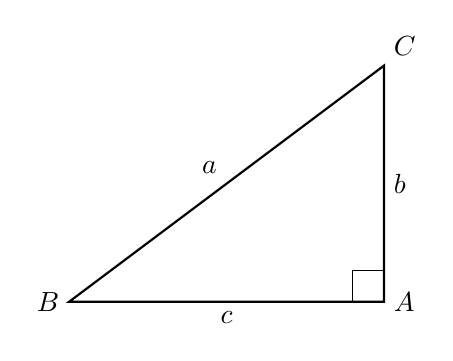
\begin{tikzpicture}
    % Pontos do triângulo
    \coordinate (B) at (0,0);
    \coordinate (A) at (4,0);
    \coordinate (C) at (4,3);

    % Lados do triângulo
    \draw[thick] (B) -- (A) -- (C) -- cycle;

    % Marcação do ângulo reto em B
    \draw (A) ++(-0.4,0) -- ++(0,0.4) -- ++(0.4,0);

    % Nome dos vértices
    \node[right] at (A) {$A$};
    \node[left] at (B) {$B$};
    \node[above right] at (C) {$C$};

    % Lados a, b, c
    \path (B) -- node[above left] {$a$} (C);
    \path (A) -- node[right] {$b$} (C);
    \path (A) -- node[below] {$c$} (B);

    \end{tikzpicture}
    \caption{Triângulo retângulo.}
\end{figure}
